As has been discussed in the previous sections, we are interested in visualizing
and understanding the difference in performance between predictive and
horizontal auto-scaling for one pod initialization time and four
different traffic patterns. As such, we have four different tests on which we
compare ERU and QoS: step-ladder traffic pattern with 135s pod initialization
time, jagged-edge traffic pattern with 135s pod initialization time,
increase-decrease traffic pattern with 135s pod
initialization time and flash-crowd traffic pattern with 135s pod initialization time.

For each test on the matrix, we provide two different sources of information.
First, we generate a graph comparing the summation of ERU and QoS across the
evaluation time for predictive and reactive auto-scaling. Additionally,
we provide statistical measurements for the difference of predictive and
reactive auto-scaling at the same point in the evaluation sequence (i.e. we
compare the summation of ERU and QoS after 10 minutes for predictive with the
summation of ERU and QoS after 10 minutes for reactive). With respect to
statistical measurements, we calculate a one-sided p-value
based on the null hypothesis that the difference
between the summation of ERU and QoS for predictive and reactive auto-scaling is
$0$. As we are interested in seeing if predictive auto-scaling performs better
than reactive auto-scaling, we calculate a one-sided p-value, $p$, with the alternative
hypothesis that the difference between the summation of ERU and QoS for
predictive and reactive auto-scaling is greater than $0$. We test for
significance at the $5\%$ significance level, meaning that if $p < 0.05$, we can
reject our null hypothesis in favor of our alternative hypothesis that
predictive auto-scaling performs better than reactive auto-scaling for this
combination of traffic pattern and pod initialization time.

\subsubsection{135s and step-ladder}

\begin{figure}[!h]
  \centerline{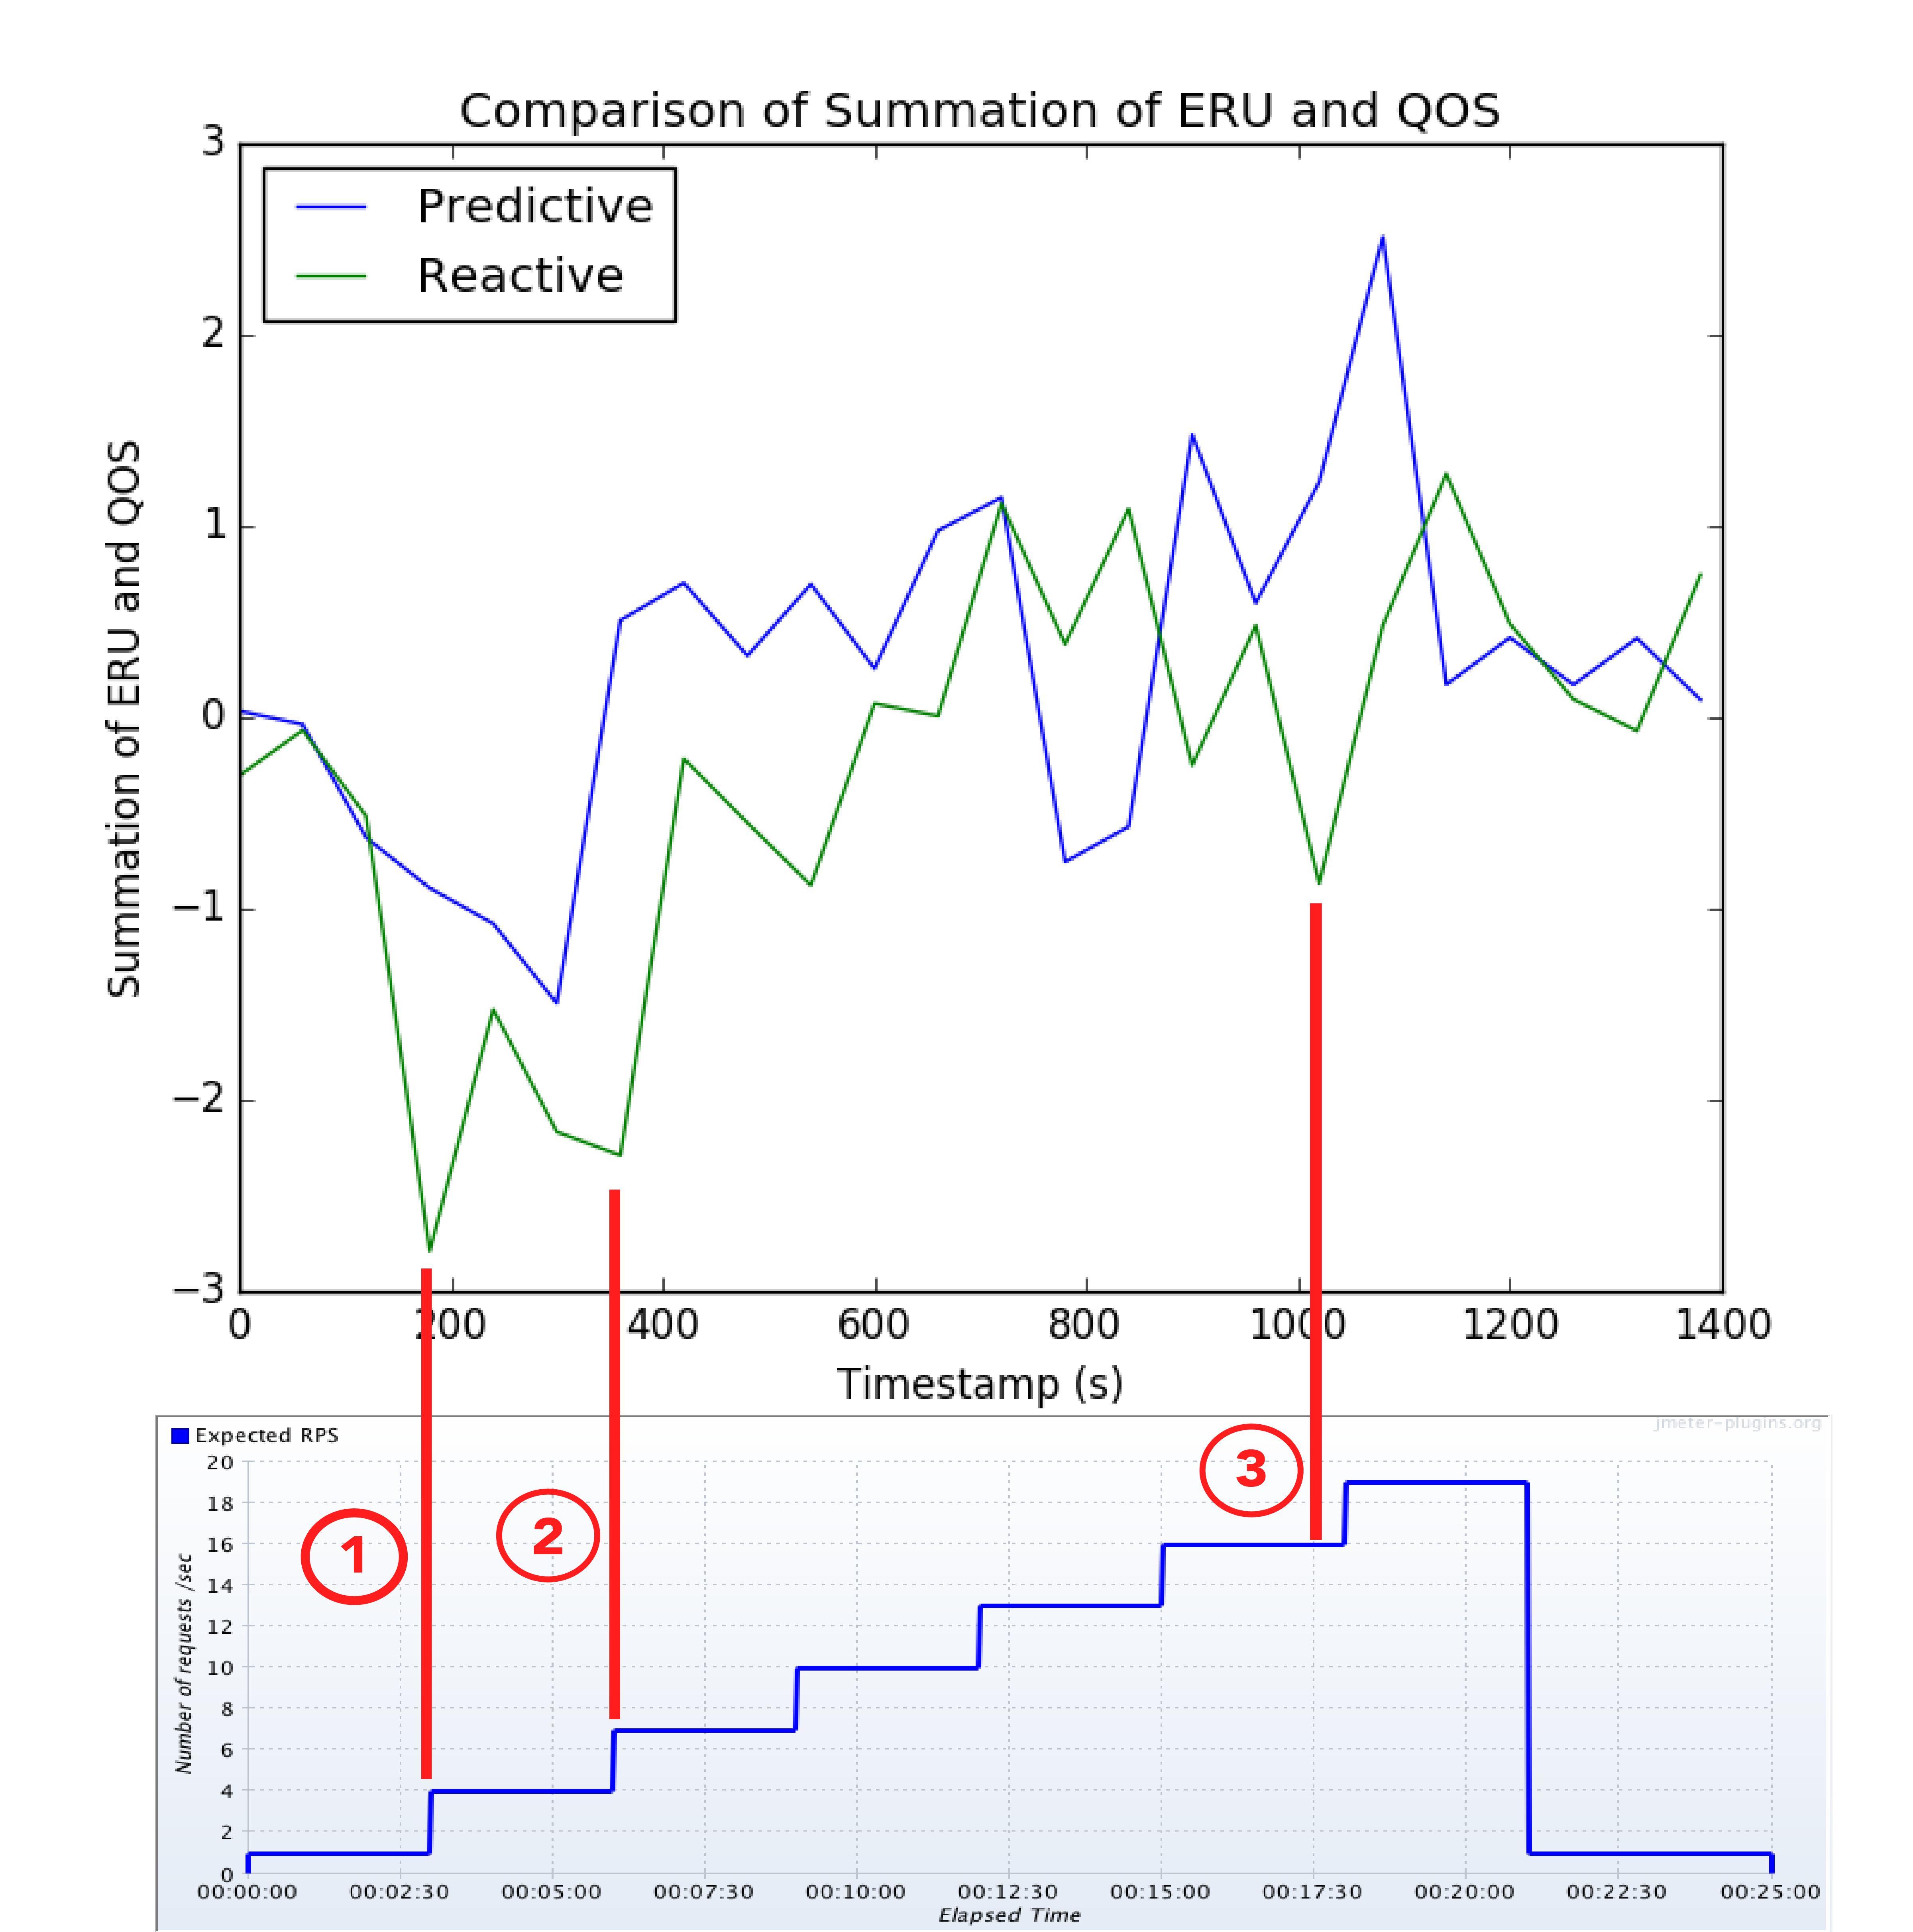
\includegraphics[scale=.70]{step-ladder-labelled.png}}
  \caption{A comparison of the summation of ERU and QoS for
    predictive and reactive auto-scaling for 135s, step-ladder.}
  \label{fig:135s-step-ladder-labelled}
\end{figure}

Figure \ref{fig:135s-step-ladder-labelled} contains a graph
showing predictive and reactive auto-scaling's different
summations of efficient resource utilization and quality of service over the
course of trial. The traffic pattern super imposed below reflects the load
placed on the sample application, indicating the effect of the traffic pattern
on the summation of ERU and QoS. Given that larger values of the summation of ERU and QoS
are more desirable, times when the predictive line rises above the reactive line
reflect moments at which predictive auto-scaling is outperforming reactive
auto-scaling. Specifically, we can see three moments, labelled $1, 2,$ and
$3$ on the graph, in which predictive auto-scaling is particularly effective in
comparison to reactive auto-scaling. These moments help reveal a true strength of
predictive auto-scaling. While reactive auto-scaling under provisions because it
purely predicts based on the current moment, predictive auto-scaling is able to
recognize the general linearly upward pattern and auto-scale accordingly. As
such, the predictively auto-scaled application always has the resources it needs
to remain performant, as can be seen when examining the comparison of just
negated QoS in Figure \ref{fig:135s-step-ladder-only-qos}.\footnote{Again,
because we negated QoS when showing this graph, the larger the negated QoS
measure, the more performant the application, so it is desirable for the
predictive line to rise above the reactive line.} Finally, there is no cost in
ERU for auto-scaling, as can be seen when we just compare ERU in Figure
\ref{fig:135s-step-ladder-only-eru}.\footnote{This observation holds true
throughout the majority of the thesis. When the summation of predictive and
reactive auto-scaling diverges, it is because of variation in QoS. ERU stays
relatively constant between the two, which is necessary because it shows QoS
improvements are not coming at the cost of decreased ERU.
Thus for the remainder of the traffic
patterns we show only the summation of ERU and QoS with the understanding that
predominately QoS is contributing.} Overall, the included graphs clearly
demonstrate the benefits of predictive auto-scaling for this traffic pattern.

\begin{figure}[!tbp]
  \centering
  \begin{minipage}[b]{0.4\textwidth}
    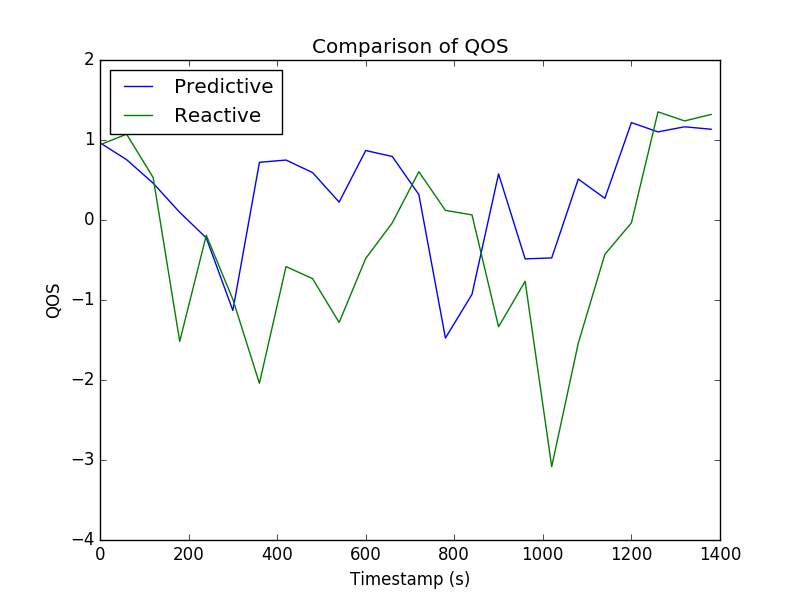
\includegraphics[width=\textwidth]{graph_135s_step-ladder_v2_only-qos.png}
    \caption{A comparison of negated QoS for predictive and reactive
    auto-scaling for 135s, step-ladder.}
    \label{fig:135s-step-ladder-only-qos}
  \end{minipage}
  \hfill
  \begin{minipage}[b]{0.4\textwidth}
    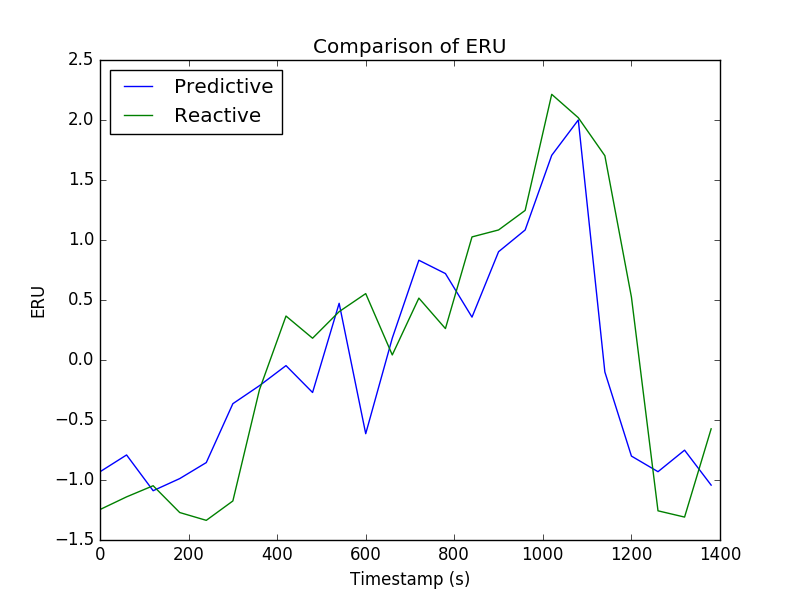
\includegraphics[width=\textwidth]{graph_135s_step-ladder_v2_only-eru.png}
    \caption{A comparison of negated ERU for predictive and reactive
    auto-scaling for 135s, step-ladder.}
    \label{fig:135s-step-ladder-only-eru}
  \end{minipage}
\end{figure}

\begin{table}[!b]
  \centering
  \caption{Difference in Predictive and Reactive Auto-scaling for 135s,
  step-ladder.}
  \label{tab:135s-step-ladder}
\begin{tabular}{l c}\hline\hline
    \multicolumn{1}{c}{\textbf{Measure}} & \textbf{Value} \\ \hline
     p-value & 0.315 \\
     z-score & 0.482 \\
     std\_dev & 1.084 \\
     mean & 0.522
  \end{tabular}
\end{table}

While Figure \ref{fig:135s-step-ladder-labelled} shows the benefits of predictive
auto-scaling on the \textit{step-ladder} traffic pattern,
we are additionally interested in knowing if said benefits are
statistically significant.
As can be seen from the summary statistics in Table \ref{tab:135s-step-ladder},
with a p-value of .315 we are not
able to reject our null hypothesis that there is no difference between the
summation of ERU and QoS for predictive and reactive auto-scaling in favor of
our alternative hypothesis that there is a positive difference in the summation
of ERU and QoS for predictive and reactive auto-scaling. Essentially, this
p-value indicates that if there was truly no difference between predictive and
reactive auto-scaling, we could expect to get these results about three out of
ten times we ran trials. Additionally, for the remainder of our trials with
different traffic patterns we were unable to obtain statistical significance.
This lack of statistical significance is likely the result of too little data,
given that we only ran one trial for each traffic-pattern, instead of combining
the results of multiple trials. Additionally, it may also be the case that the
inclusion of buffer periods, and periods when the requests per second are
sufficiently low such that only one pod needs to exist, mutes the
differences that occur when auto-scaling begins.


\subsubsection{135s and jagged-edge}

\begin{figure}[!h]
  \centerline{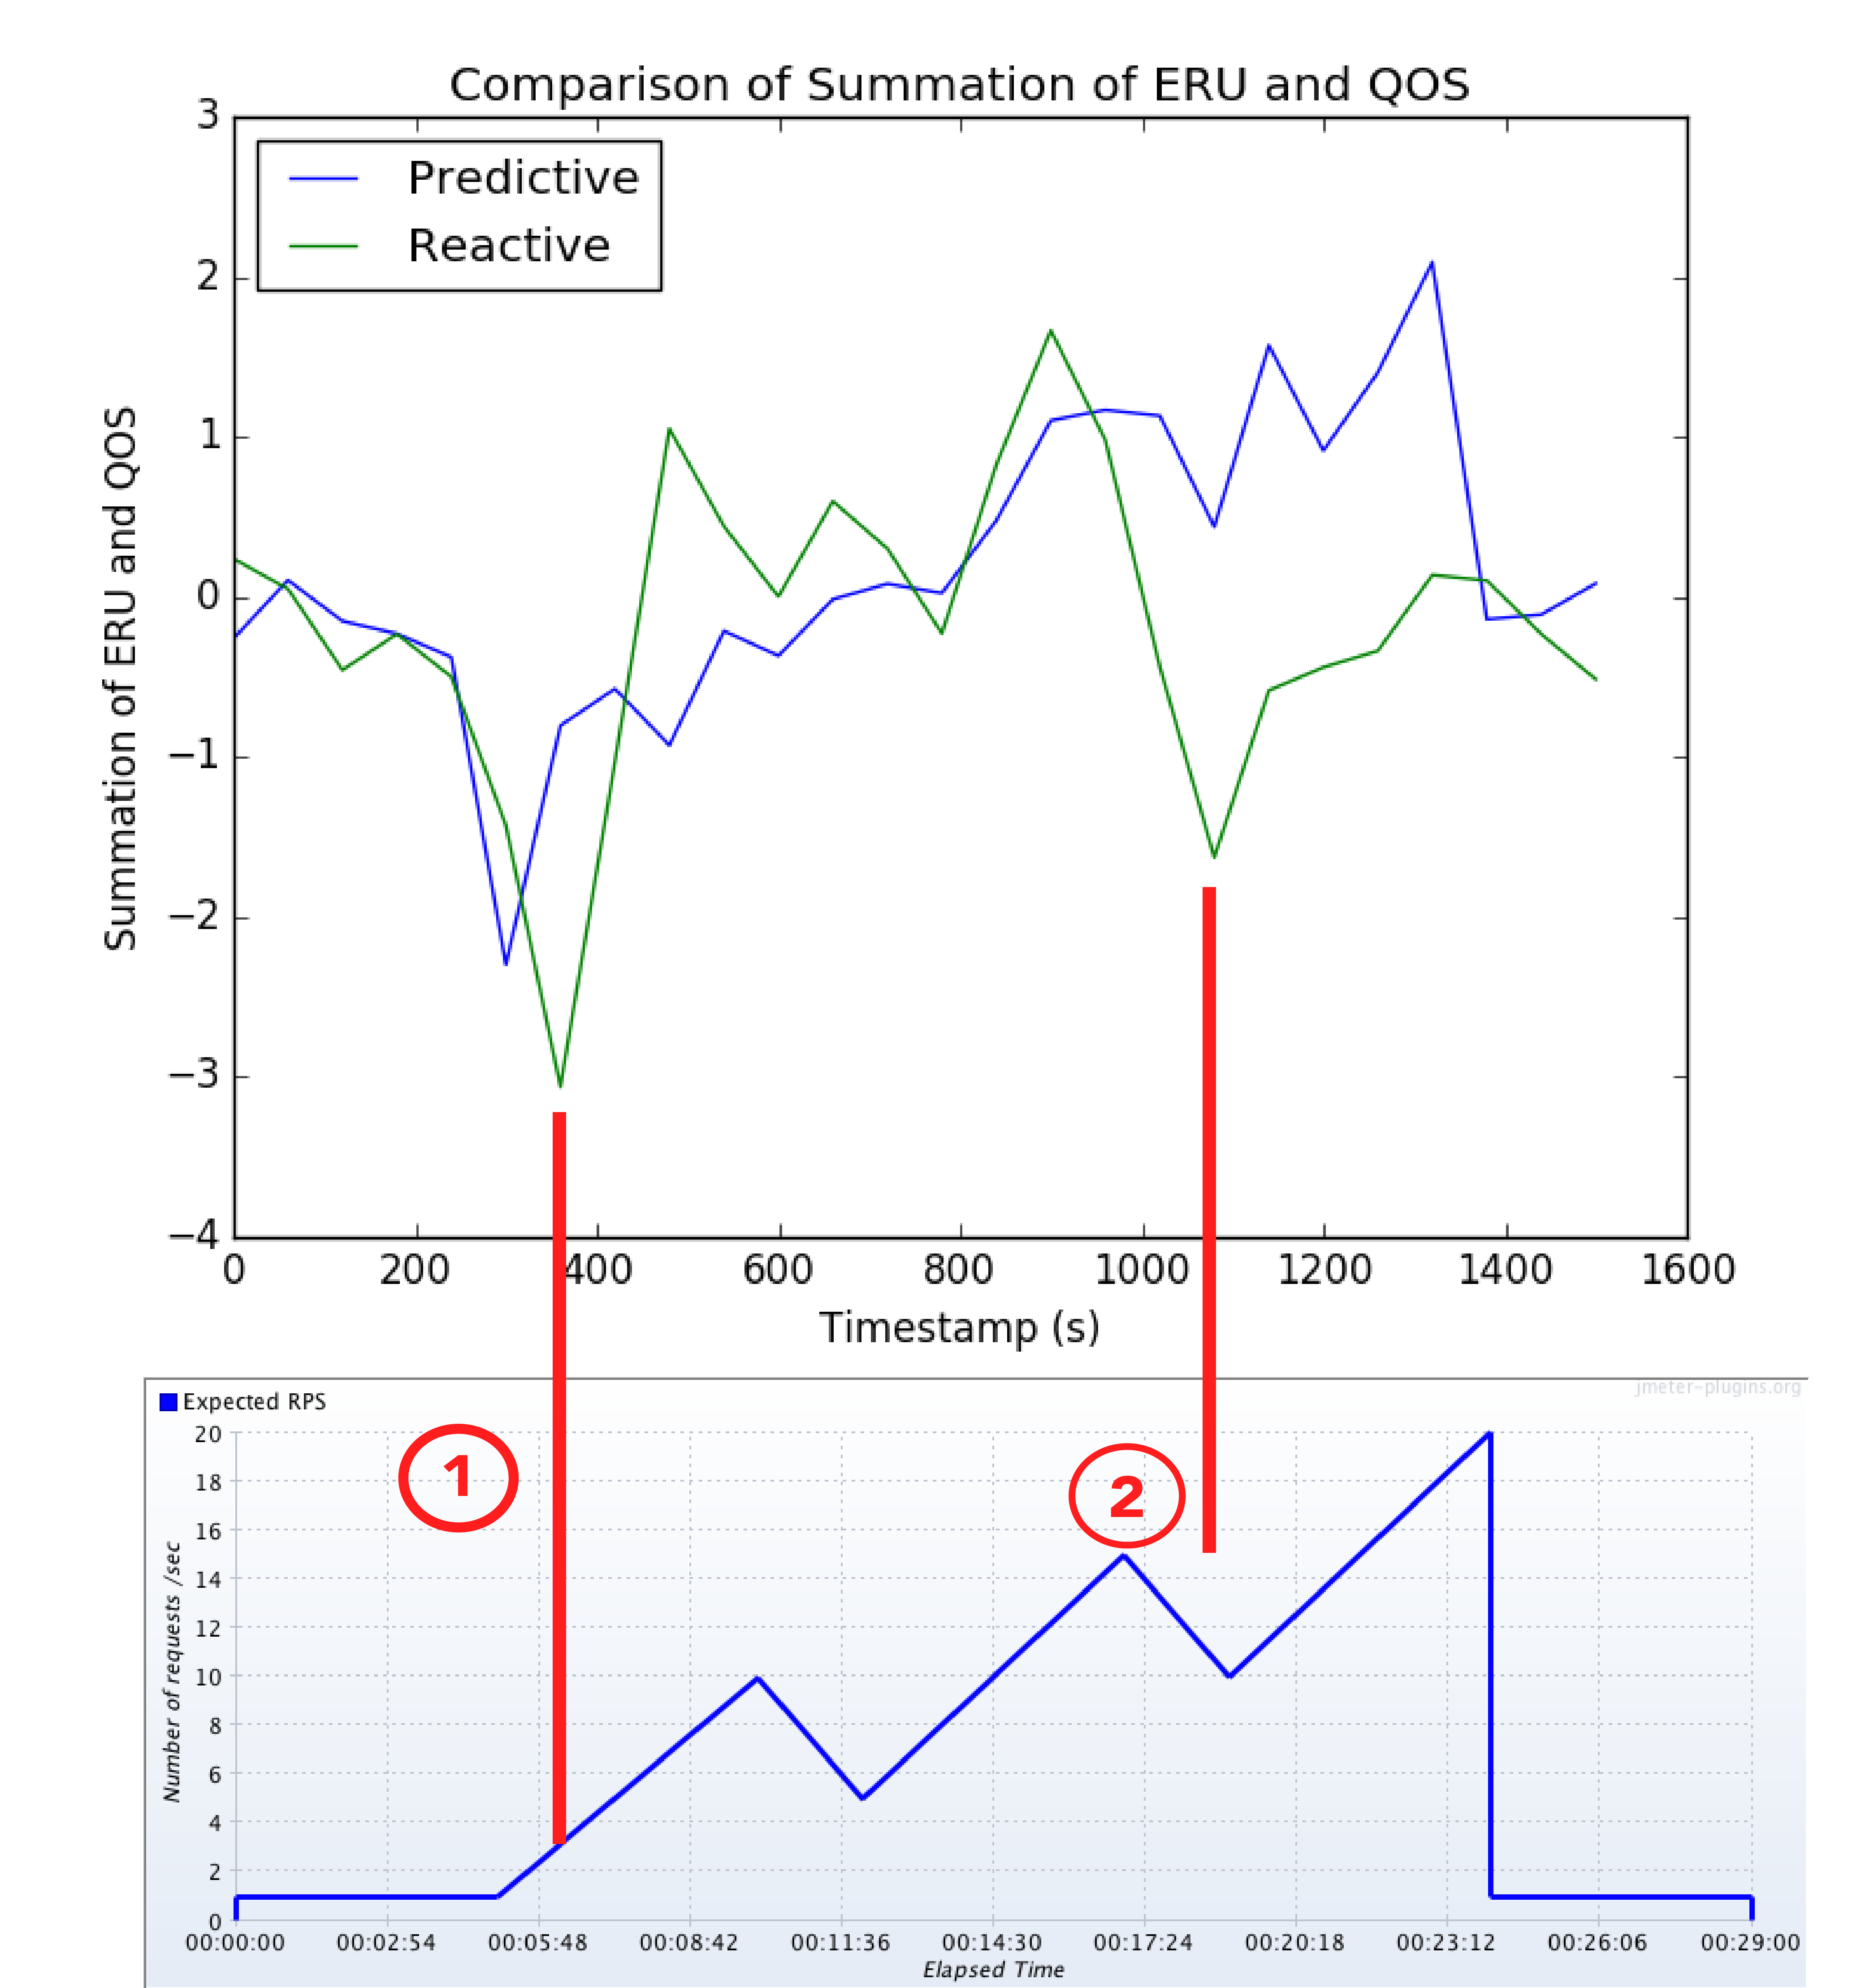
\includegraphics[scale=.70]{jagged-edge-labelled.png}}
  \caption{A comparison of the summation of ERU and QoS for
    predictive and reactive auto-scaling for 135s, jagged-edge.}
  \label{fig:135s-jagged-edge-labelled}
\end{figure}


Figure \ref{fig:135s-jagged-edge-labelled} contains a graph
showing predictive and reactive auto-scaling's different
summations of efficient resource utilization and quality of service over the
course of the \textit{jagged-edge} trial.
The traffic pattern super imposed below reflects the load
placed on the sample application, indicating the effect of the traffic pattern
on the summation of ERU and QoS. Again, we highlight significant times, labelled
$1$ and $2$ for which
predictive auto-scaling has a higher summation of ERU and QoS, and as such is
outperforming reactive auto-scaling. The decrease in the summation of ERU and
QoS for reactive auto-scaling, labelled with the $2$ on the graph, again
reflects the advantages of predictive auto-scaling's ability to understand the
general linear pattern and not drastically under-provision as the result of
temporary downturns.

\begin{table}[htbp]
  \centering
  \caption{Difference in Predictive and Reactive Auto-scaling for 135s,
  jagged-edge.}
  \label{tab:135s-jagged-edge}
\begin{tabular}{l c}\hline\hline
    \multicolumn{1}{c}{\textbf{Measure}} & \textbf{Value} \\ \hline
     p-value & 0.374 \\
     z-score & 0.320 \\
     std\_dev & 1.062 \\
     mean & 0.340
  \end{tabular}
\end{table}

Similarly, while Figure \ref{fig:135s-jagged-edge-labelled} shows the benefits of predictive
auto-scaling on the \textit{jagged-edge} traffic pattern, Table
\ref{tab:135s-jagged-edge} shows that we are unfortunately not able to claim
statistical significance with respect to these results.


\subsubsection{135s and increase-decrease}

\begin{figure}[!h]
  \centerline{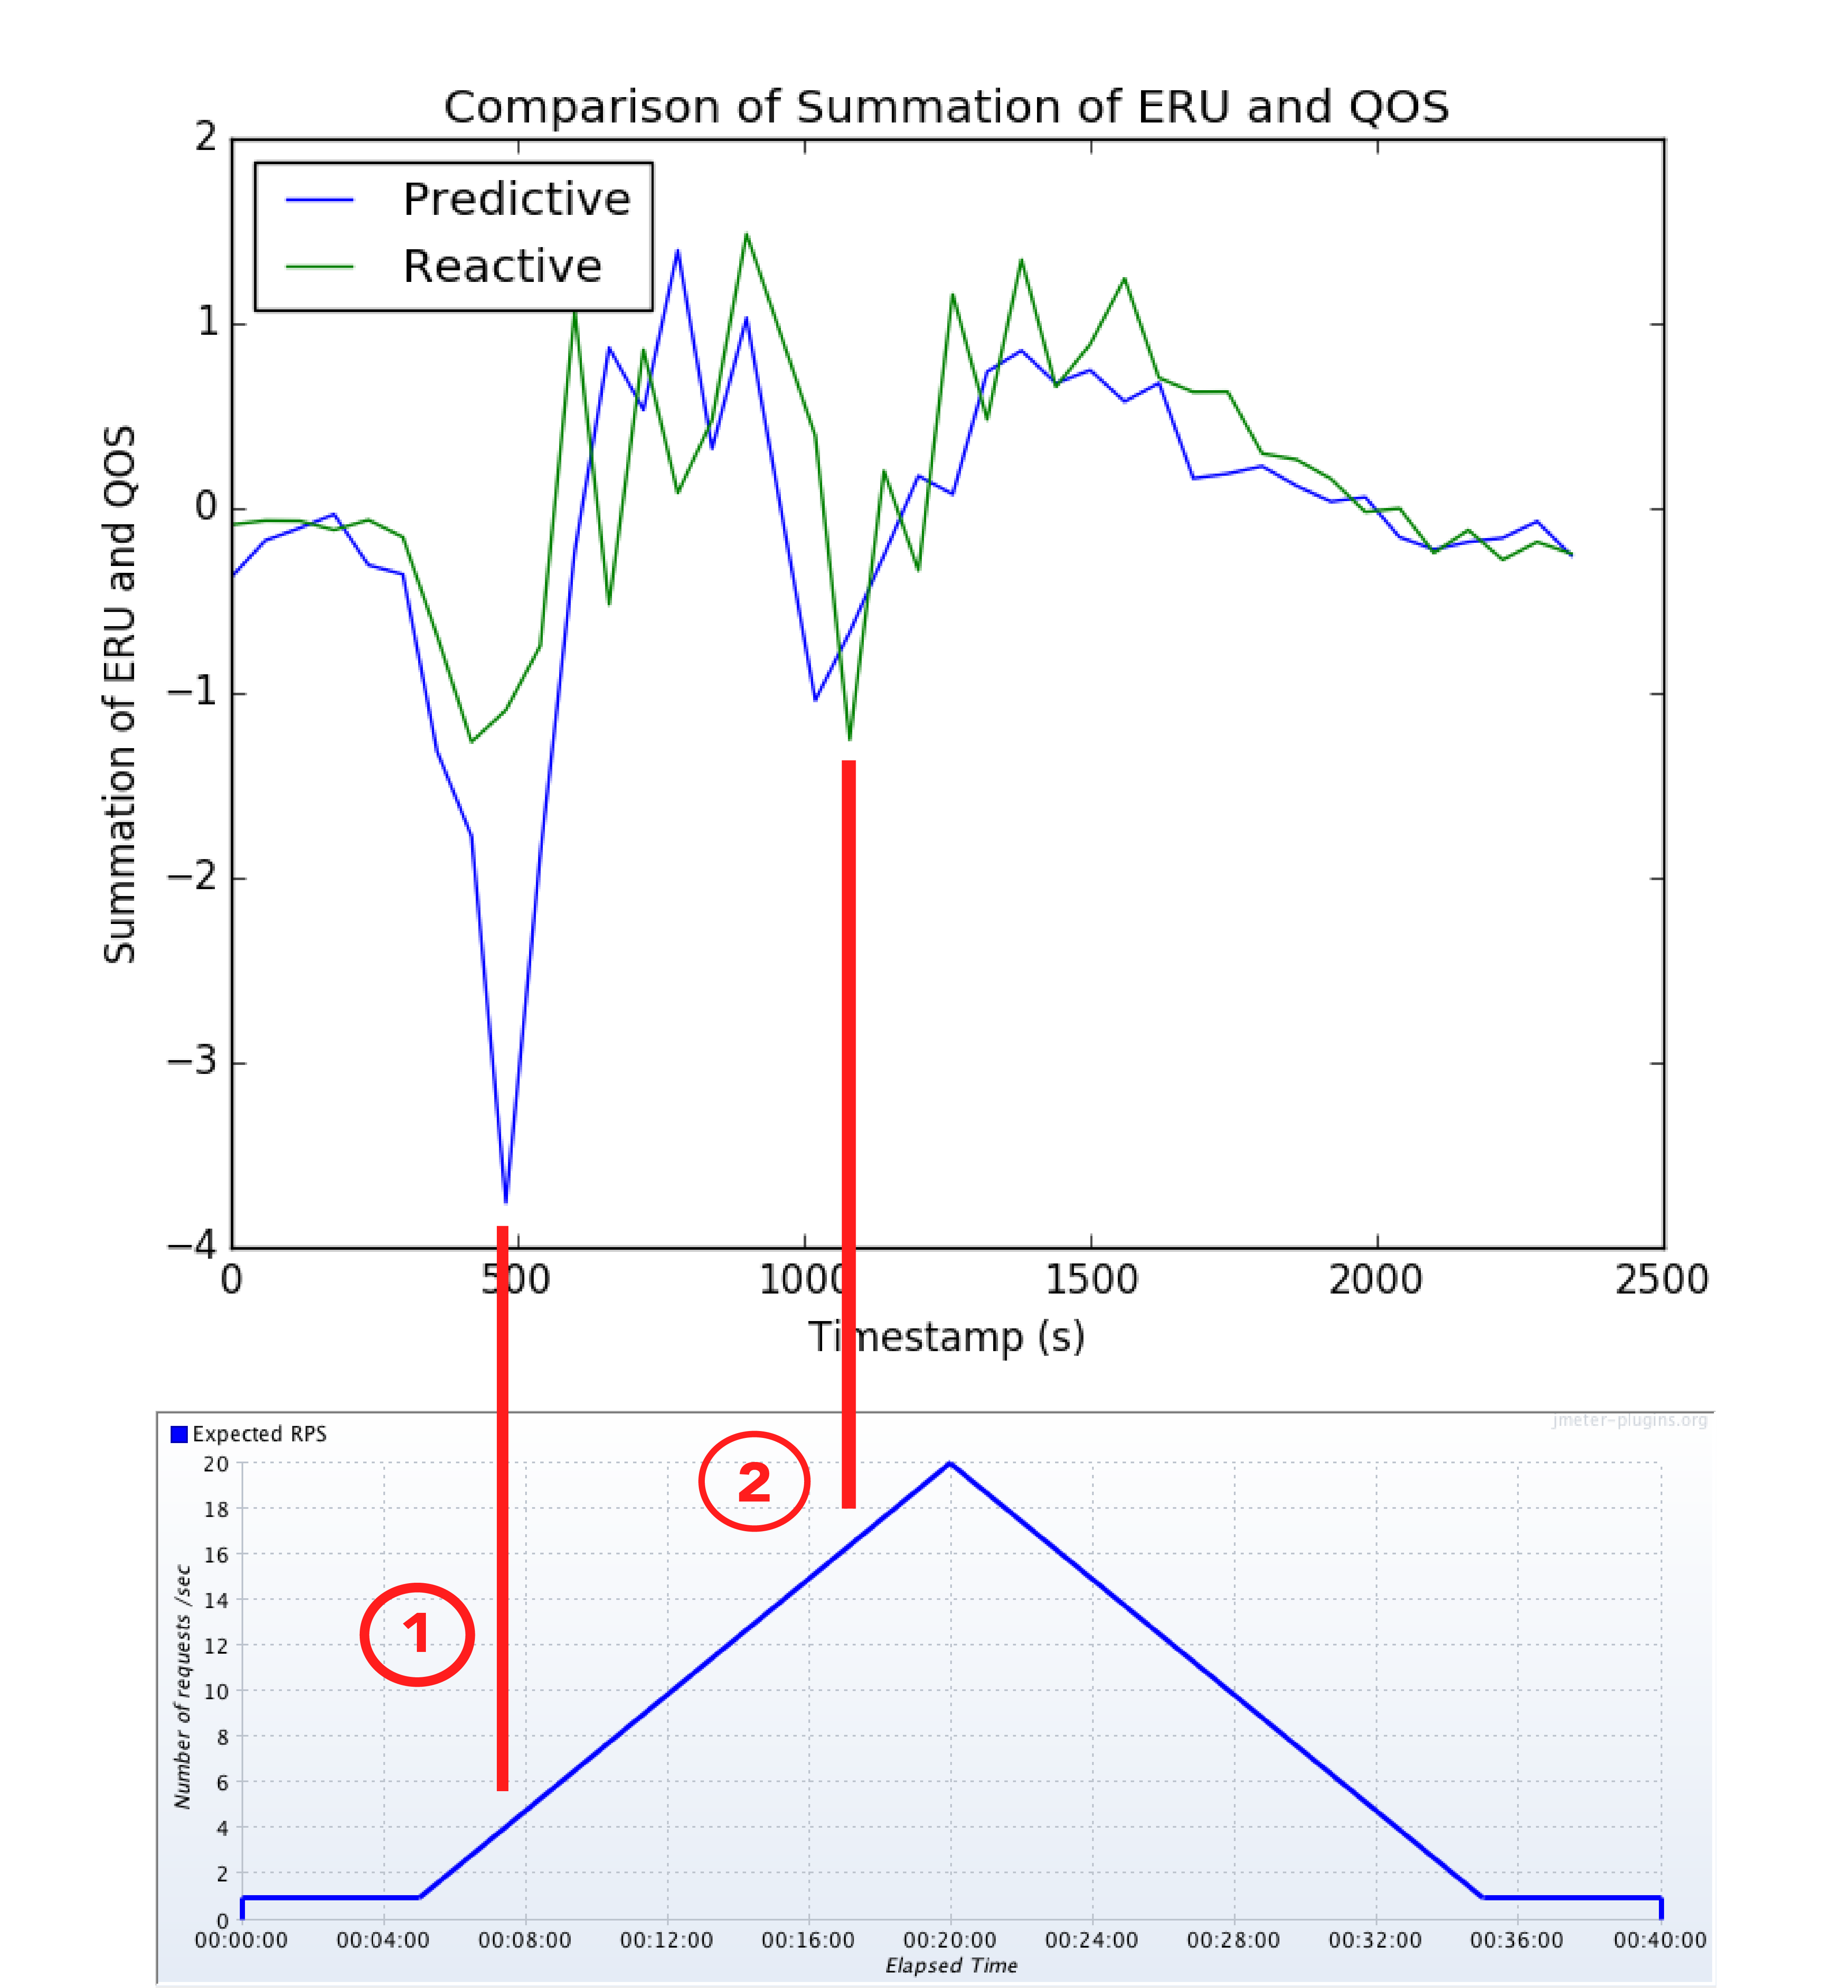
\includegraphics[scale=.70]{increase-decrease-labelled.png}}
  \caption{A comparison of the summation of ERU and QoS for
    predictive and reactive auto-scaling for 135s, increase-decrease.}
  \label{fig:135s-increase-decrease-labelled}
\end{figure}

Figure \ref{fig:135s-increase-decrease-labelled} contains a graph
showing predictive and reactive auto-scaling's different
summations of efficient resource utilization and quality of service over the
course of the \textit{increase-decrease} trial. In contrast to our previous two
traffic patterns, we find that predictive auto-scaling is not particularly
beneficial in this context. Specifically, if we look at the moment labelled
$1$ on Figure \ref{fig:135s-increase-decrease-labelled}, we an instance in which
predictive auto-scaling suffers a severe performance decrease in comparison to
reactive auto-scaling. We trace this decrease again to under-provisioning. In
this scenario, the introductory buffer period has caused our linear prediction
algorithm to underestimate the slope of the line indicating the rise in load. As
such, the reactive auto-scaling algorithm actually has a more aggressive opinion
of the load the application will face. As this aggressive understanding is
confirmed by our actual increase, reactive auto-scaling outperforms predictive
auto-scaling on the \textit{increase-decrease} traffic-pattern. Scenario
$1$ is in contrast to the scenario labelled $2$, in which predictive
auto-scaling performs equally to reactive auto-scaling, because it is no longer
negatively impacted by previous measurements which do not reflect the current
slope.

\begin{table}[htbp]
  \centering
  \caption{Difference in Predictive and Reactive Auto-scaling for 135s,
  increase-decrease.}
  \label{tab:135s-increase-decrease}
\begin{tabular}{l c}\hline\hline
    \multicolumn{1}{c}{\textbf{Measure}} & \textbf{Value} \\ \hline
     p-value & 0.638 \\
     z-score & -.0352 \\
     std\_dev & 0.680 \\
     mean & -0.234
  \end{tabular}
\end{table}

Figure \ref{fig:135s-increase-decrease-labelled} shows that predictive
auto-scaling is actually slightly detrimental on
the \textit{increase-decrease} traffic pattern.
Still, Table \ref{tab:135s-increase-decrease} shows that we are not able to claim
statistical significance with respect to these results, and thus should not be
too confident that prediction has a negative effect. Rather, it appears to
have very little impact in either direction on this traffic pattern.


\subsubsection{135s and flash-crowd}

\begin{figure}[!h]
  \centerline{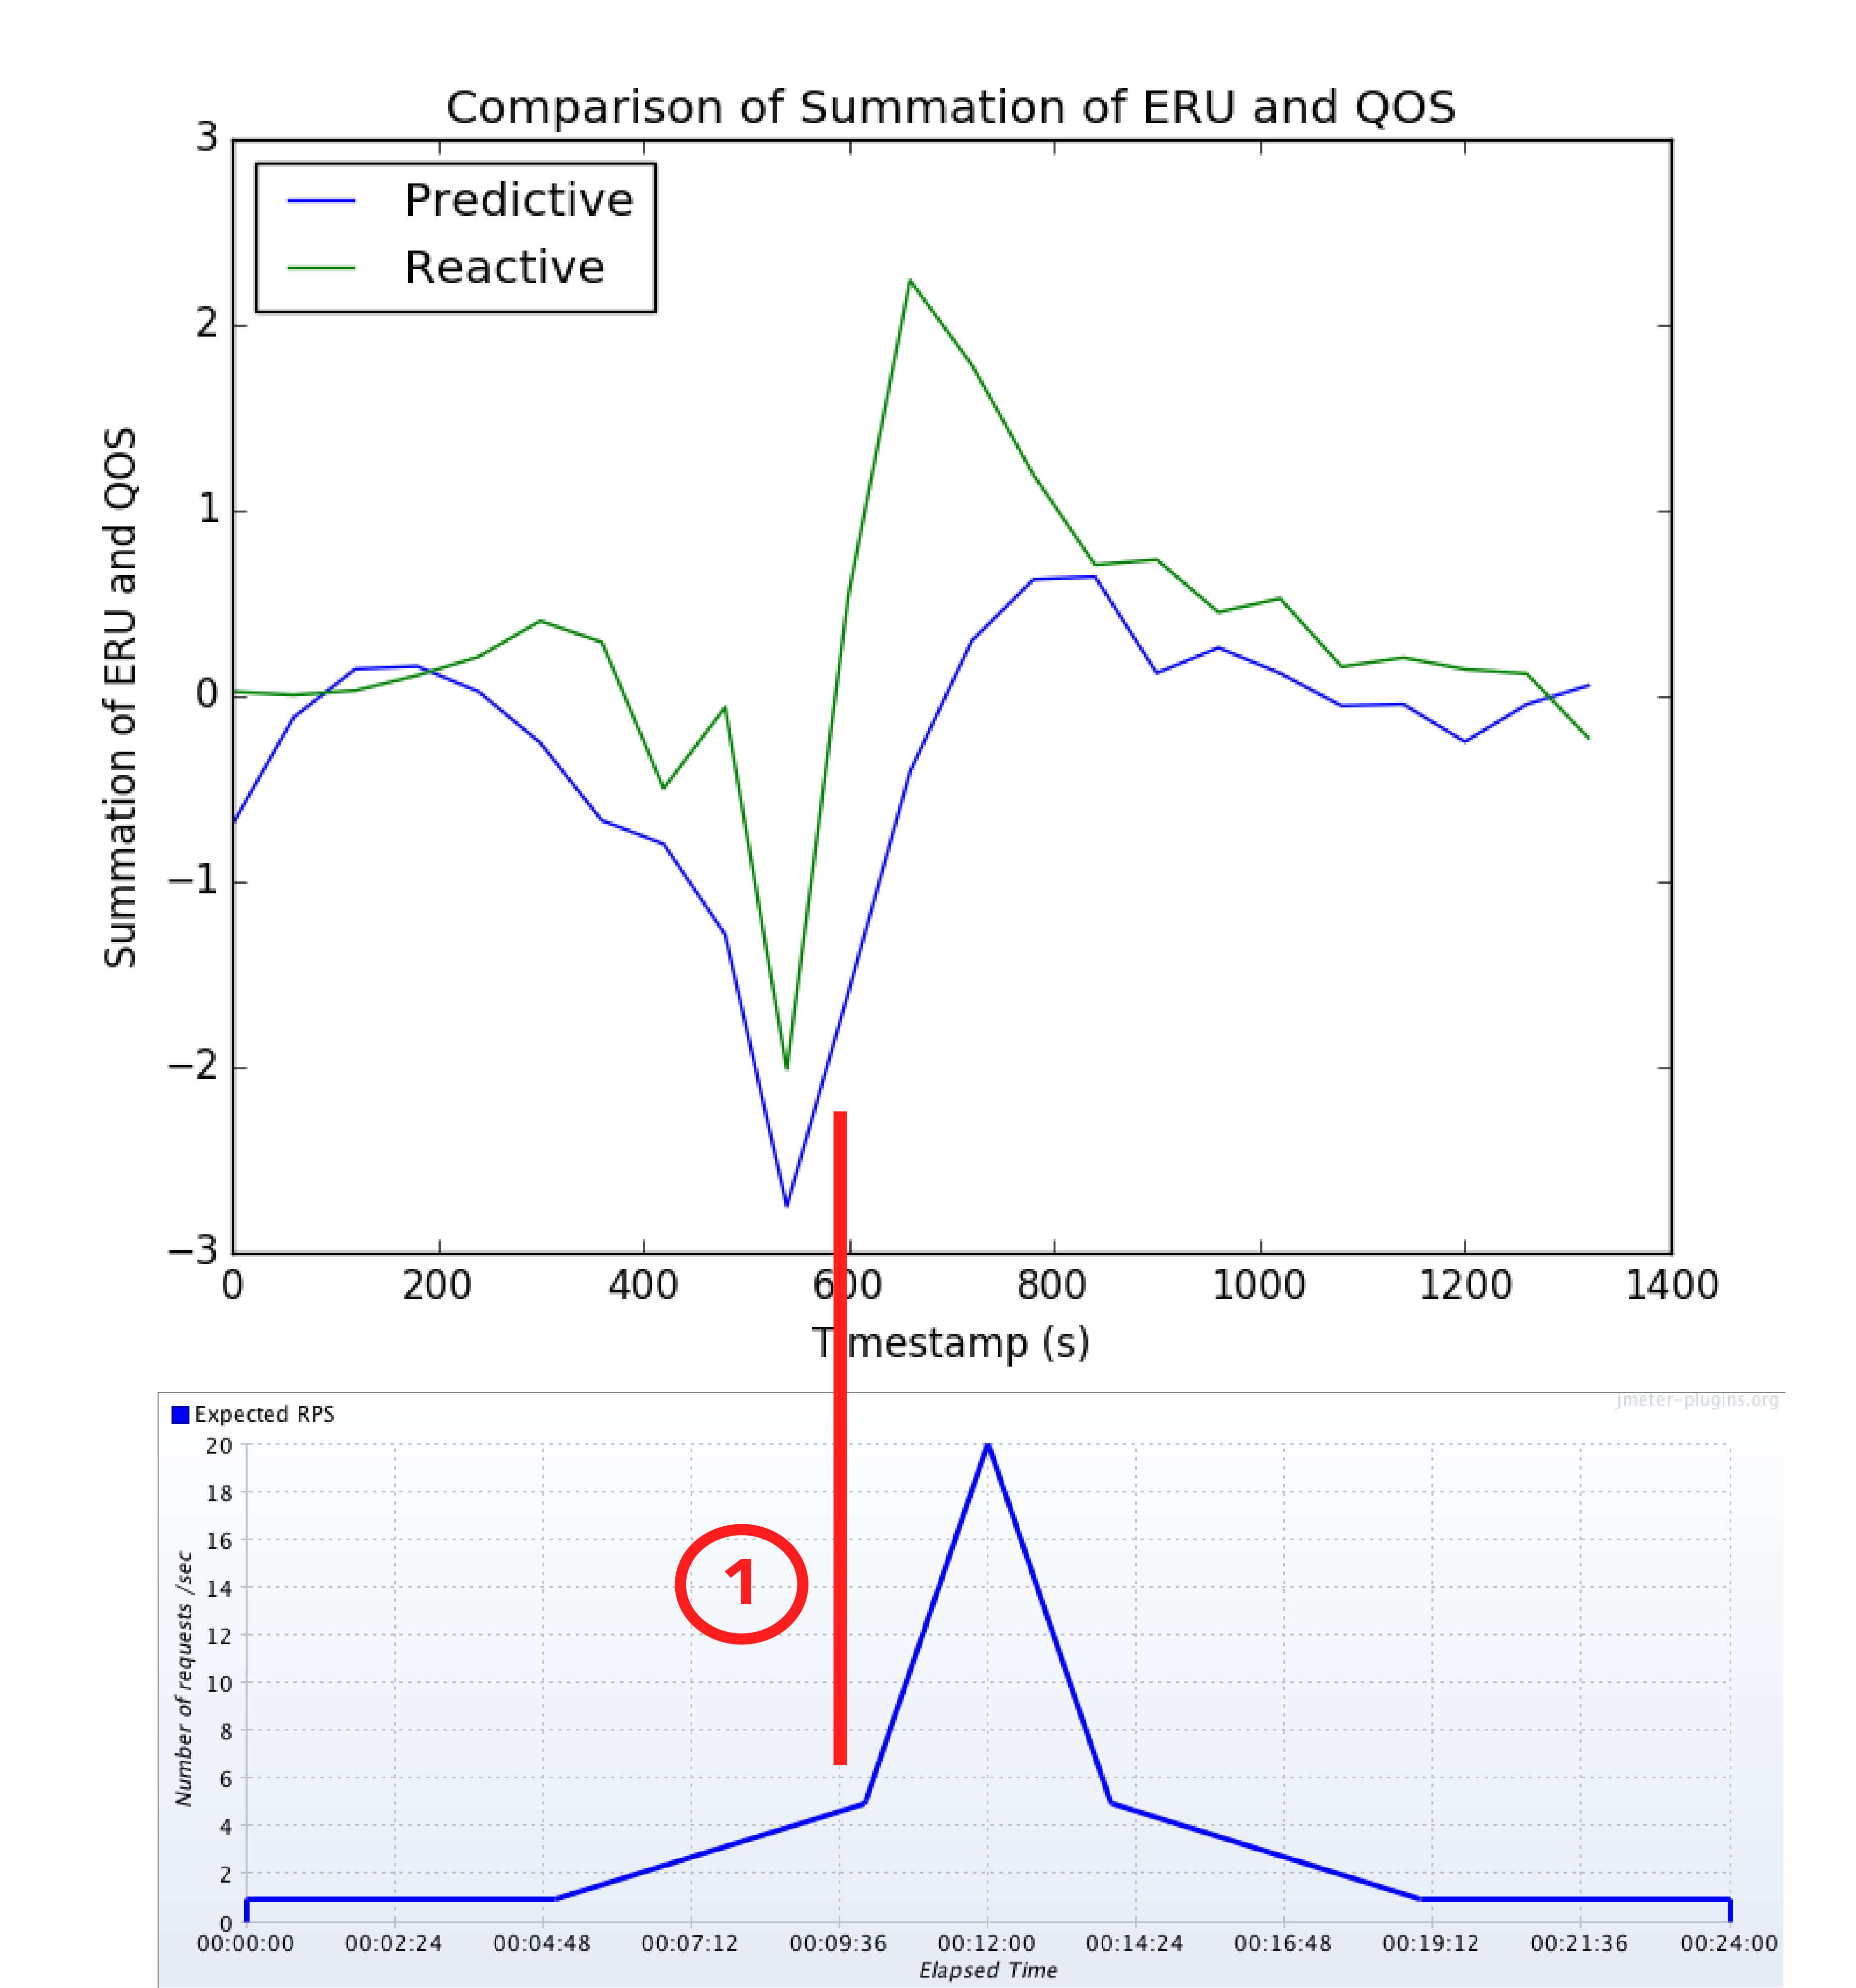
\includegraphics[scale=.70]{flash-crowd-short-labelled.png}}
  \caption{A comparison of the summation of ERU and QoS for
    predictive and reactive auto-scaling for 135s, flash-crowd.}
  \label{fig:135s-flash-crowd-labelled}
\end{figure}

Figure \ref{fig:135s-flash-crowd-labelled} contains a graph
showing predictive and reactive auto-scaling's different
summations of efficient resource utilization and quality of service over the
course of the \textit{flash-crowd} trial. Again,
we find that predictive auto-scaling is not particularly
beneficial in this context. Specifically, if we look at the moment labelled
$1$ on Figure \ref{fig:135s-flash-crowd-labelled}, we see another instance in which
predictive auto-scaling suffers a severe performance decrease because of
under-provisioning. Because this traffic pattern occurs over such a short
interval, the predictive auto-scaling algorithm is unable to fully recognize and
respond to the flash crowd, and is instead hampered by previous measurements
with a significantly lesser slope. Our line-of-best-fit for prediction has too
small a slope, and thus predictive auto-scaling functions worse than reactive
auto-scaling.

\begin{table}[htbp]
  \centering
  \caption{Difference in Predictive and Reactive Auto-scaling for 135s,
  flash-crowd.}
  \label{tab:135s-flash-crowd}
\begin{tabular}{l c}\hline\hline
    \multicolumn{1}{c}{\textbf{Measure}} & \textbf{Value} \\ \hline
     p-value & 0.802 \\
     z-score & -.850 \\
     std\_dev & 0.695 \\
     mean & -0.591
  \end{tabular}
\end{table}

Figure \ref{fig:135s-flash-crowd-labelled} shows that predictive
auto-scaling is fairly detrimental on the \textit{flash-crowd} traffic pattern.
Given Table \ref{tab:135s-flash-crowd}, we are still not able to claim
statistical significance with respect to these results, but we should be fairly
confident that this current iteration of predictive auto-scaling is not an advisable addition
when expecting flash crowds.

